\documentclass[a4paper,12pt]{report}

\usepackage{alltt, fancyvrb, url}
\usepackage{graphicx}
\usepackage[utf8]{inputenc}
\usepackage{float}
\usepackage{xcolor}
\usepackage{hyperref}

% Questo commentalo se vuoi scrivere in inglese.
\usepackage[italian]{babel}

\usepackage[italian]{cleveref}

\title{Elaborato per il corso di\\''Programmazione di Reti''}
\author{Rebosio Alessandro}
\date{\today}

\begin{document}

\maketitle

\tableofcontents

\chapter{Introduzione}

L'obiettivo di questo progetto è la realizzazione di un \textbf{server HTTP} \newline minimale sviluppato in \textbf{Python},
capace di gestire richieste di tipo GET sulla porta 8080 di localhost e di servire contenuti statici
in formato HTML e CSS.

\vspace{0.5cm}

Il progetto intende fornire una comprensione pratica del protocollo HTTP, dell'utilizzo dei \textbf{socket}
per la comunicazione di rete e del funzionamento di base di un \textbf{web server}.

\vspace{0.5cm}

Attraverso la realizzazione di un server costruito manualmente, è stato possibile esplorare in modo diretto e
applicato i concetti fondamentali delle reti e della programmazione di basso livello.

\subsubsection{Funzionalità principali}
\begin{itemize}
    \item Risposta con codice di stato 200 per risorse esistenti;
    \item Gestione dell'errore 404 per risorse non trovate;
    \item Riconoscimento e gestione dei MIME types per i file serviti;
    \item Logging delle richieste ricevute;
    \item Pubblicazione di un sito web statico composto da tre pagine HTML responsive.
\end{itemize}

\chapter{Archittetura del progetto}
L'architettura del progetto si basa su una suddivisione tra la logica applicativa del server e i
contenuti statici da servire al client.

\section{Descrizione dell'architettura}
\begin{itemize}
    \item \textbf{src/server.py}: implementa il web server HTTP, ascolta sulla porta 8080 e serve file
          statici presenti nella cartella \texttt{www/}.
    \item \textbf{www/}: contiene il sito web statico, costituito da tre pagine HTML e un file CSS
          condiviso. Le pagine includono layout responsive e contenuti base.
\end{itemize}

\begin{figure}[H]
    \centering
    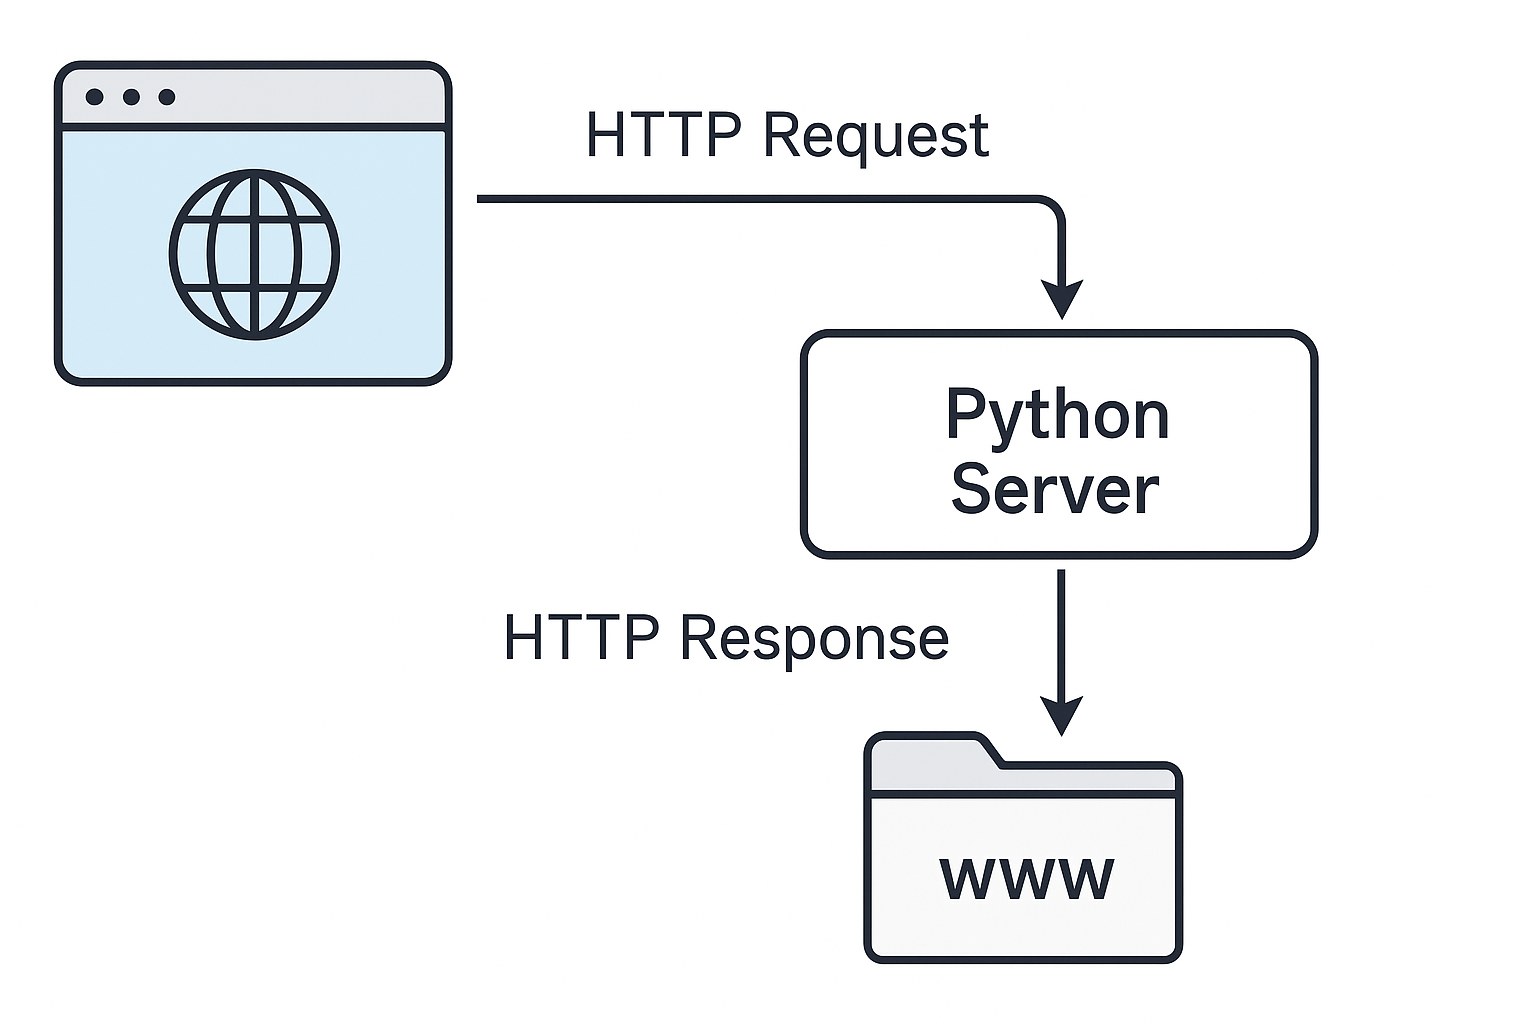
\includegraphics[width=0.5\textwidth]{img/architettura.png}
    \caption{Schema dell'architettura client-server}
    \label{fig:architettura}
\end{figure}

In \Cref{fig:architettura} viene rappresenta l'interazione tra browser, server e file system. Quando un client
invia una richiesta HTTP, il server interpreta la richiesta, individua il file richiesto nella directory \texttt{www/}
e restituisce il contenuto.

\chapter{Implementazione del web server}
L'implementazione del server HTTP è interamente in \texttt{Python} utilizzando il modulo \texttt{socket} per
la comunicazione e il modulo \texttt{threading} per la gestione concorrente delle connessioni.

\section{Struttura generale}
\begin{itemize}
    \item \textbf{HTTPServer}: classe usata per stabilire una o più connessioni \newline attraverso la creazione di
          un \texttt{socket}, che viene poi associato alla \texttt{porta 8080} per accettare le connessioni in ingresso.
    \item \textbf{HTTRequestHandler}: classe per il parsing delle richieste con il successivo invio di risposte.
    \item \textbf{MyServer}: sottoclasse per semplificare la logica, nella quale viene implementato il
          metodo \texttt{do\_GET} per servire i file richiesti dai client.
\end{itemize}

\section{Gestione delle richieste}
Quando un client tenta la connessione e viene accettata, il server crea un nuovo \texttt{thread} per gestirla, permettendo
le richieste in modo concorrente.

La richiesta viene letta, vengono estratti il \texttt{metodo}, \texttt{path} e la versione \texttt{HTTP} dalla prima
riga.

Successivamente se la risorsa richiesta esite nella directory \texttt{www/}, viene caricata e restituita la risposta
con il codice \texttt{(200, OK)}. Altrimenti viene restituita la risposta di errore con il codice \texttt{(404, Not Found)}.

\section{Gestione MIME types e logging}
Il server usa la libreria \texttt{mimestype} per determinare il tipo di contenuto da servire in base all'estensione del
file.

Ogni \texttt{richiesta} viene loggata \Cref{fig:logging} in console con il formato: indirizzo IP del client, data e ora, metodo, risorsa richiesta
e codice di stato restituito.

\subsubsection{Esempi di logging:}
\begin{figure}[H]
    \centering
    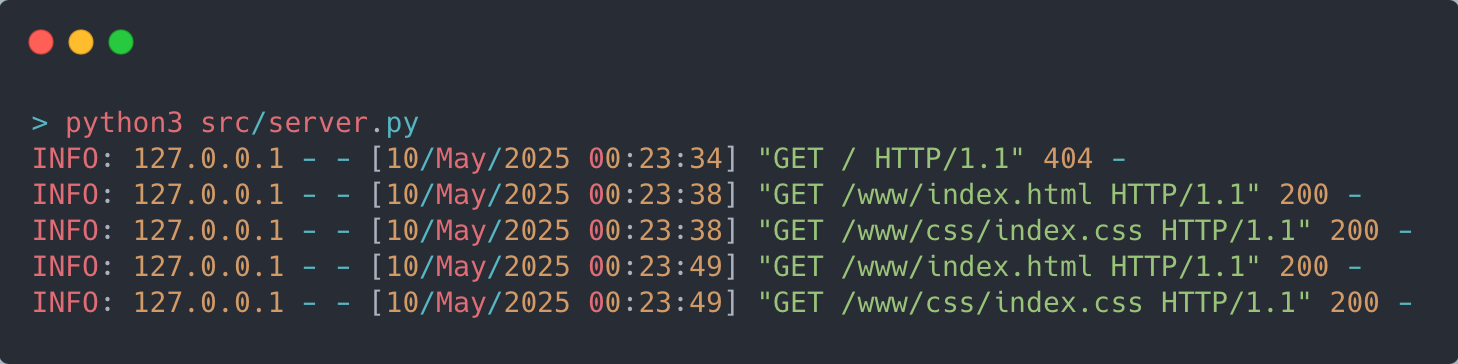
\includegraphics[width=1\textwidth]{img/logging.png}
    \caption{Log delle richieste in console}
    \label{fig:logging}
\end{figure}

\section{Sicurezza base}

Per evitare accessi non autorizzati a file esterni alla cartella \texttt{www/}, il \newline path richiesto viene sanificato
rimuovendo sequenze potenzialmente pericolose come \texttt{../}.

\subsubsection{Sicurezza del path:}
\begin{figure}[H]
    \centering
    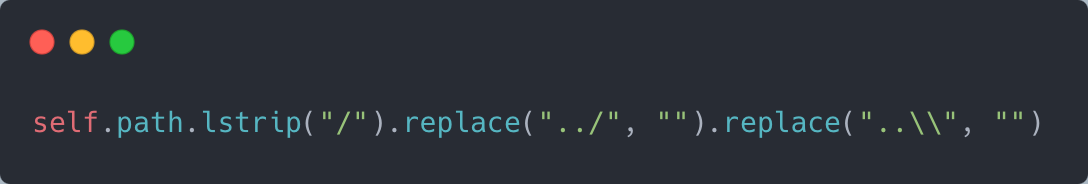
\includegraphics[width=1\textwidth]{img/safe_path.png}
    \caption{Codice per path sicura}
    \label{fig:safe_path}
\end{figure}


\chapter{Sito web statico}

\chapter{Test e risultati}

\chapter{Conclusioni}

\chapter{Appendice}

\end{document}
